\begin{frame}
    \frametitle{BlockChain Overview}
    \begin{itemize}
        \item The block chain provides Bitcoin's public ledger, an ordered and timestamped record of transctions.
        \item This system is used to protect against double spending and modification of previous transactions records.
        \item Each full node in the Bitcoin network independently stores a block chain containing only blocks validated by that node.
    \end{itemize}
    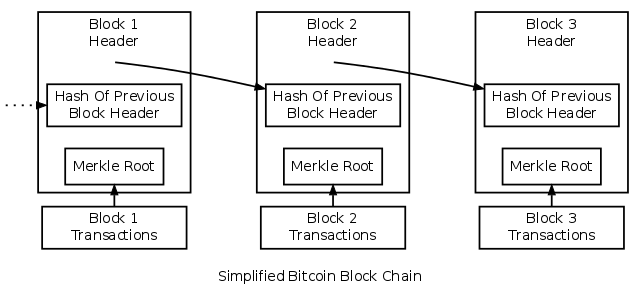
\includegraphics[scale=0.4]{en-blockchain-overview.png}
\end{frame}

\begin{frame}[fragile]
    \frametitle{BlockChain Data Structure}
    \begin{columns}
        \begin{column}{0.6\textwidth}
            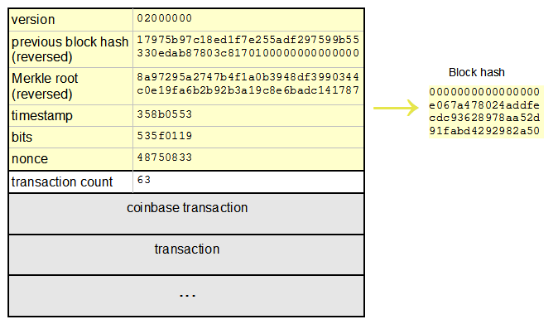
\includegraphics[scale=0.5]{blockchain-data-structure.png}
        \end{column}
        \begin{column}{0.4\textwidth}
            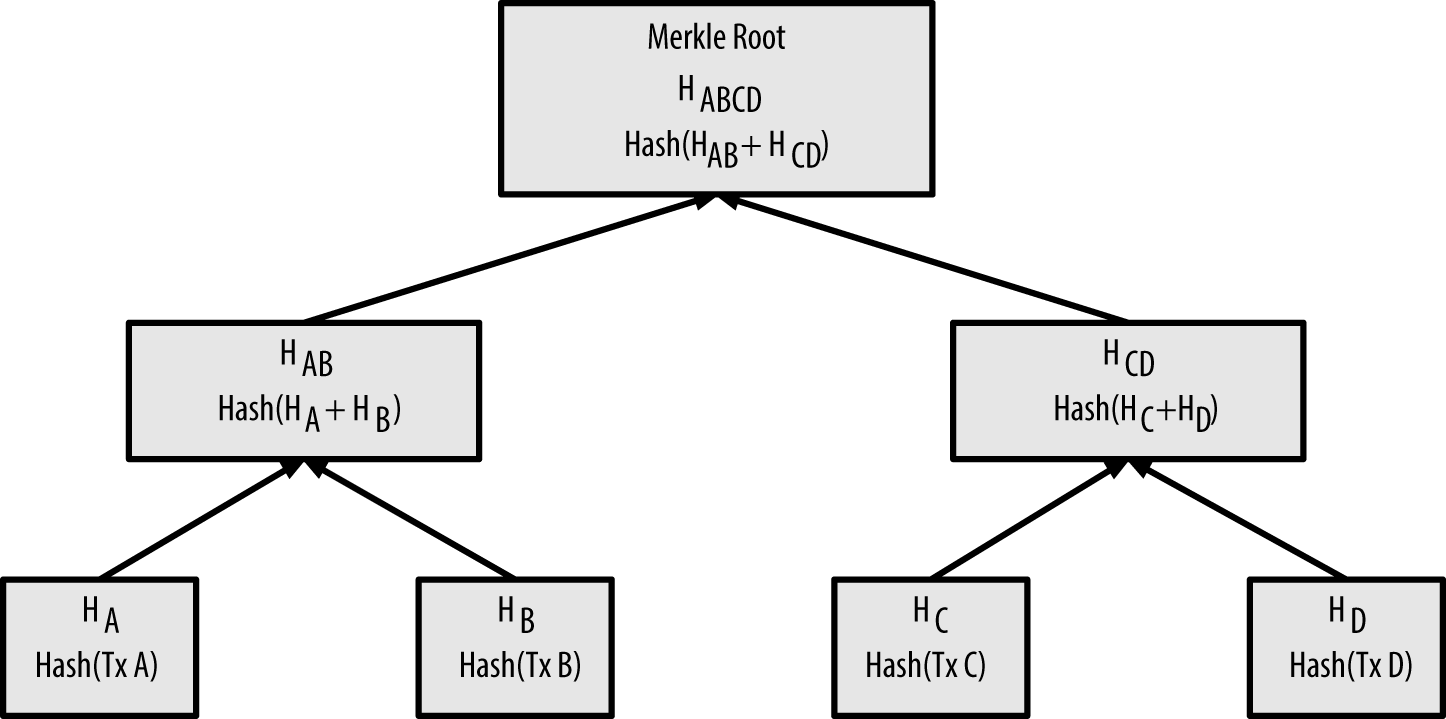
\includegraphics[scale=0.4]{mbc2_0902.png}
        \end{column}
    \end{columns}
    \begin{itemize}
        \item \textbf{Block Header}: 80 bytes, whereas transctions is at least 250 bytes.
        \item \textbf{Nonce}: A counter used for proof-of-work algorithm.
        \item \textbf{Difficulty}: How difficult it is to find a hash below a given target.
        \item \textbf{Coinbase}: The content of the \alert{input} of a generation transction.
    \end{itemize}
    \begin{lstlisting}[language=Python]
The Times 03/Jan/2009 Chancellor on brink of second bailout for banks. \end{lstlisting}
\end{frame}

\begin{frame}[fragile]
    \frametitle{The Genesis Block}
    \begin{lstlisting}[language=Python]
bitcoind getblock 000000000019d6689c085ae165831e934ff763ae46a2a6c172b3f1b60a8ce26f
{
    "hash" : "000000000019d6689c085ae165831e934ff763ae46a2a6c172b3f1b60a8ce26f",
    "confirmations" : 308321,
    "size" : 285,
    "height" : 0,
    "version" : 1,
    "merkleroot" : "4a5e1e4baab89f3a32518a88c31bc87f618f76673e2cc77ab2127b7afdeda33b",
    "tx" : [
        "4a5e1e4baab89f3a32518a88c31bc87f618f76673e2cc77ab2127b7afdeda33b"
    ],
    "time" : 1231006505,
    "nonce" : 2083236893,
    "bits" : "1d00ffff",
    "difficulty" : 1.00000000,
    "nextblockhash" : "00000000839a8e6886ab5951d76f411475428afc90947ee320161bbf18eb6048"
}
    \end{lstlisting}
    The difficulty value updates every 2 weeks to ensure that it takes 10 minutes(on average) to add a new block to the BlockChain.
    \begin{lstlisting}[language=Python]
0x00ffff * 2**(8*(0x1d-3))=0x00000000FFFF0000000000000000000000000000000000000000000000000000 \end{lstlisting}
\end{frame}

\begin{frame}[fragile]
    \frametitle{Proof Of Work}
    \begin{itemize}
        \item Block contains transctions to be validated and previous hash value.
        \item Pick a nonce such that \textbf{H(prev hash, nonce, Tx) < E}.
        \item Verification is easy, But proof-of-work is hard.
    \end{itemize}
    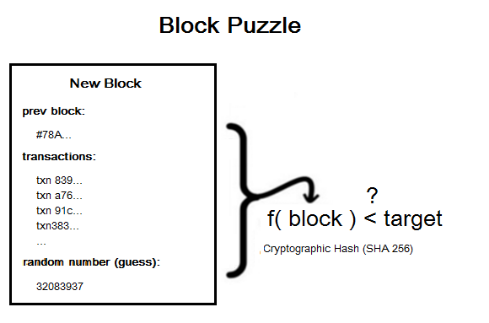
\includegraphics[scale=0.5]{block-puzzle.png}
\end{frame}

\begin{frame}[fragile]
    \frametitle{Difficulty Target and Re-Target}
    Every 2016 blocks, all node re-target the Proof-of-Work difficulty.
    \begin{lstlisting}[language=Python]
New Difficulty = Old Difficulty * (20160 minutes / Actual Time of Last 2016 Blocks)
The Target = The maximum target / current difficulty.
The maximum target is:
    0x00000000FFFF0000000000000000000000000000000000000000000000000000 \end{lstlisting}

    Re-Target Code in bitcoind
    \begin{lstlisting}[language=C++]
    // Limit adjustment step
    int64_t nActualTimespan = pindexLast->GetBlockTime() - nFirstBlockTime;
    LogPrintf("  nActualTimespan = %d  before bounds\n", nActualTimespan);
    if (nActualTimespan < params.nPowTargetTimespan/4)
        nActualTimespan = params.nPowTargetTimespan/4;
    if (nActualTimespan > params.nPowTargetTimespan*4)
        nActualTimespan = params.nPowTargetTimespan*4;

    // Retarget
    const arith_uint256 bnPowLimit = UintToArith256(params.powLimit);
    arith_uint256 bnNew;
    arith_uint256 bnOld;
    bnNew.SetCompact(pindexLast->nBits);
    bnOld = bnNew;
    bnNew *= nActualTimespan;
    bnNew /= params.nPowTargetTimespan;

    if (bnNew > bnPowLimit)
        bnNew = bnPowLimit; \end{lstlisting}
\end{frame}
